\documentclass[tikz,border=2mm]{standalone}
\usetikzlibrary{calc,quotes,intersections, angles}

\begin{document}
    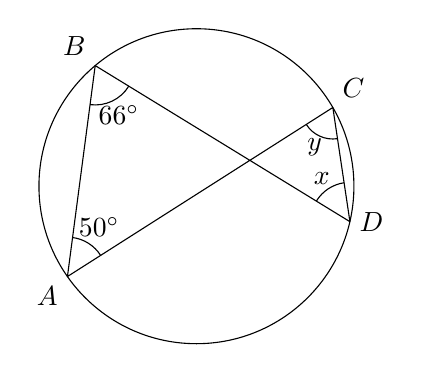
\begin{tikzpicture}[scale=2]
    
        \coordinate[label=above left:$B$] (B) at (130:1);
        \coordinate[label=below left:$A$] (A) at (215:1);
        \draw[name path=circ] (0,0) circle (1);
        \path[name path=BD] (B) -- ($(B)!1.5!66:(A)$);
        \path[name path=AC] (A) -- ($(A)!1.5!-50:(B)$);
        \path[name intersections={of=circ and BD, by={[]K,D}}];
        \path[name intersections={of=AC and circ, by={[label=above right:$C$]C}}];
        \draw[line join=bevel] (A) -- (B) -- (D) -- (C) -- cycle;
        \node at (D) [right] {$D$};

        \pic [draw, "$66^\circ$", angle eccentricity=1.4, angle radius = 0.5cm] {angle = A--B--D};
        \pic [draw, "$50^\circ$", angle eccentricity=1.5, angle radius = 0.5cm] {angle = C--A--B};
        \pic [draw, "$y$", angle eccentricity=1.4, angle radius = 0.4cm] {angle = A--C--D};
        \pic [draw, "$x$", angle eccentricity=1.3, angle radius = 0.5cm] {angle = C--D--B};
        
    \end{tikzpicture}

    
\end{document}